% Chapter Template

\chapter{Introduction} 
\label{chapter-introduction} 

%----------------------------------------------------------------------------------------
%	SECTION 
%----------------------------------------------------------------------------------------

\section{Motivation}

In recent years, there has been tremendous advances in the field of Artificial Intelligence (AI), especially in Deep Learning \citep{lecun-dl, deeplearning-overview}. Deep Learning has helped AI systems reach and sometimes surpass human-level perception, mostly in computer vision \citep{image-recognition} and natural language processing \citep{machine-translation}. Giving rise to multiple amazing industrial application such as autonomous driving, early cancer detection, better machine translation, etc. However, industrials often face a difficult problem during the deployment of AI in the real-world: how to make sure these systems can handle unexpected situations correctly? New deep learning models are usually tested in conditions relatively similar to those in which the models where trained, leading to an overestimation of their robustness. Indeed, inputs of the model in real-world scenarios could be missing, subject to variable noises or unseen (e.g. a dog-cat image classifier receiving an image of a fish). These kind of inputs generally degrade the quality of predictions because the inputs do not contain enough information (missing) or the information cannot be processed (too noisy or unseen).

A possible remedy to the above problem is to use multiple modalities. Our experience of the world is multi-modal, i.e., we see objects, hear sound, feel the texture, smell odours, and taste flavours. A modality, also called mode, refers to a representation with very different statistics than the other modalities in the setting \citep{taxomany-multimodal}. Multi-Modal Deep Learning (MMDL) is used in the hope is that the information carried by each mode is additive, as a result the model has more information to learn to make more accurate and more robust predictions. Impressive works has been done in this domain. Authors in \citep{afouras} created an AI performing speech-to-text using not only audio of the speaker but also video of the lip movements, achieving state-of-the art results on unconstrained natural language sentences from British television. They also investigated to what extent lip reading is complementary to noisy audio signal, showing robustness was indeed improved. In a like manner, research in self-driving cars started exploring ways to combine sensorial inputs from wide angle cameras and LIDAR\footnote{Laser Detection and Ranging} sensors for road detection \citep{lidar-camera}. An example of the representation obtained by these sensors is shown in Figure \ref{fig:lidar-camera}. Cameras provide dense information over a long range under good illumination and fair weather. Whereas LIDARs are only marginally affected by the external lighting conditions and provide accurate distance measurements but have a limited range. Fusing sensorial information with deep learning is done to get the best of both sensors. Despite the progress made, noisy and unseen modes are still fed into the mode and thus potentially perturbing the predictions. Not to mention that combining modalities is challenging due to modalities having different quantitative influence over the prediction output and having different levels of noise. 

On the other hand, humans seem to handle these situations robustly on a daily basis. A famous example showing this is called the cocktail-party effect \citep{cocktail-party}, it refers to the difficulty we sometimes have understanding speech in noisy social settings. As a subconscious response, we tend to look at the mouth of our interlocutor i.e. we shift some attention from the auditory to the visual senses. The visual stimuli is then processed by the brain, now able to more easily extract the speaker from the audio. Similarly, our attention is shifted from vision to touch when we are wandering in a room where the lights suddenly switch off. These examples demonstrate that humans are able to handle noisy, missing and unseen modes by focusing its attention smoothly on the most relevant mode(s). In this work I introduce a novel attention mechanism, named \textit{Energy-based Multi-Modal Attention} (EMMA), mimicking human's multi-modal attention. More specifically, EMMA decides how much attention to devote to each mode, such that the relevant information is kept while masking out the perturbations.
\begin{figure}[!ht]
\centering
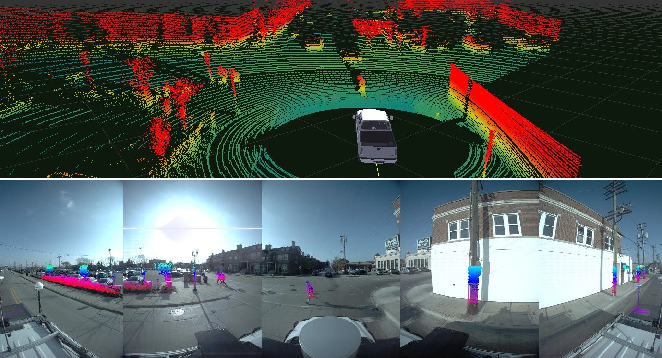
\includegraphics[scale=0.55]{figures/lidar-camera}
\caption[Lidar \& Camera view in self-driving cars]{Same environment, different modes (top: LIDAR view, bottom: camera view)}	
\label{fig:lidar-camera}
\end{figure}


%----------------------------------------------------------------------------------------
%	SECTION 
%----------------------------------------------------------------------------------------

\section{Proposed solution}
An example of how EMMA is used is illustrated in Figure \ref{fig:main-idea}. The attention module is inserted in front of the model, focusing attention on the best modes of the sample. The less outlying a mode, the more information of the mode EMMA will let pass by. We denote outlyingness as a general notion for noisiness, missing and unseen values. Additionally, EMMA takes into account how each mode contributes differently to the accuracy, and the kind of information between a pair of modes (redundant, complementary, conflicting).
\begin{figure}[!h]
\centering
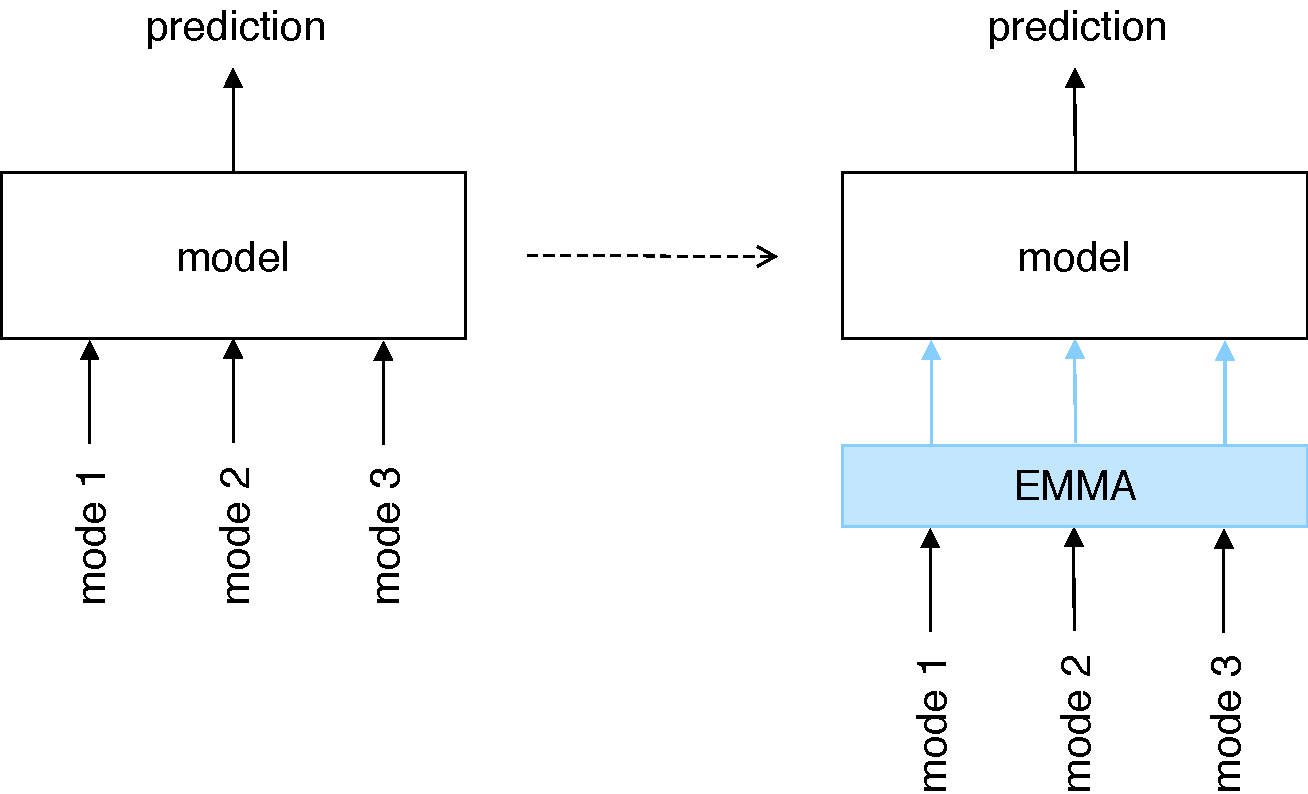
\includegraphics[scale=0.45]{figures/introduction-three-modes-with-emma}
\caption{Multi-Modal model without EMMA (left) to with EMMA (right)}	
\label{fig:main-idea}
\end{figure}

\subsection*{Hypothesis}
EMMA is constructed under the assumption that if a mode is outlying, at least one other mode can be found that is not outlying, which is thus able to "take over".

\subsection*{Software Implementation}
All the implemented models and experiments are available at this \href{https://github.com/Werenne/energy-based-multimodal-attention}{repository}\footnote{\url{https://github.com/Werenne/energy-based-multimodal-attention}}, with a wiki explaining how to run the experiments. Moreover, the main framework used regarding the Machine Learning part is \href{https://pytorch.org/}{PyTorch}\footnote{\url{https://pytorch.org/}}.

%----------------------------------------------------------------------------------------
%	SECTION 
%----------------------------------------------------------------------------------------

\section{Contributions}
The work presented in this Master thesis has led to three novel contributions.
\begin{description}
\item \textbf{Contribution 1: a module mimicking human's endogenous attention.} A new Deep Learning attention mechanism, EMMA, has been developed. It is based on Energy models \citep{EBM} to measure the outlyingness of modes and thereupon decide where to focus attention. TODO: present main results obtained.
\item \textbf{Contribution 2: a proposal for a unified model for multi-modal attention.} In Chapter \ref{chapter-background}, a review of the literature from a Psychological standpoint on attention reveals current multi-modal attention mechanisms in DL are incomplete. In Chapter \ref{chapter-unified}, an architecture for a general multi-modal attention is proposed combining EMMA and the current multi-modal attentions.
\item \textbf{Contribution 3: a constraint permitting to link capacity as in} \citep{attention-is-effort} \textbf{and deep learning attention functions.} A common parametric function for Attention in DL is slightly transformed such that it resembles more human attention. The transformation can easily be generalized to most attention functions.
\end{description}

%----------------------------------------------------------------------------------------
%	SECTION 
%----------------------------------------------------------------------------------------

\section{Thesis Outline}
The remainder of this work is organised as follows.
\begin{description}
\item \textbf{Chapter 2} explains the background this work is based upon.
\item \textbf{Chapter 3} reviews the existing literature of Multi-Modal Deep Learning, putting forward their limitations.
\item \textbf{Chapter 4} describes two ways of estimating the outlyingness of data and how these are derived.
\item \textbf{Chapter 5} presents the ideas and architecture of the Energy-based Multi-Modal Attention module (Contribution 1 \& 3).
\item \textbf{Chapter 6} presents a thorough evaluation and analysis of the module outlined in Chapter \ref{chapter-emma}.
\item \textbf{Chapter 7} from current attention mechanisms and the developed EMMA module, a more general multi-modal attention architecture is discussed (Contribution 2).
\item \textbf{Chapter 8} concludes this work and suggests possible directions for future research.
\end{description}